\chapter{РАЗРАБОТКА АЛГОРИТМА УПРАВЛЕНИЯ БУФЕРОМ КОМПЕНСАЦИИ ДЖИТТЕРА} \label{chapt:man}

Существующие телекоммуникационные системы активно используют различные методы управления: ситуационные, основанные на логике лиц, принимающих решение; автоматические; автоматизированные.
Вместе с тем, за последние годы все более процедур в телекоммуникационных сетях новых поколений осуществляется автоматически, с оптимизацией этих процедур, что позволяет за кратчайшее время получать наибольший эффект от управления данными процедурами.

В существующих технологиях большой удельный вес занимают методы управления, основанные на принципах Понселе. Данный принцип основан на предположении о том, что любому обнаруженному возмущению находится адекватное управление, реагирующее на это возмущение.
Структурная схема управления, функционирующая по принципу Понселе, показана на рис. \ref{fig:ponsele} \cite{popovski}.


\begin{figure}[!h]

\centering
\begin{tikzpicture}
[node distance = 1cm, auto,
% STYLES
every node/.style={node distance=6cm},
% The force style is used to draw the forces' name
force/.style={rectangle, draw, fill=white!10, inner sep=5pt, text width=4cm, text badly centered, minimum height=1.2cm}] 


% Draw forces
\node [force] (resolving) {Принятое решение};
\node [force, right of=resolving] (object) {Управляемый объект};

 \draw [>=latex,->] (resolving) edge node {$u(t)$} (object);
\draw [>=latex,->,densely dashed] (object)    -- +(0,-2)  -| (resolving);
\node (ask) at (3, -2.5) {Подтверждение об исполнении};

\end{tikzpicture} 
\caption{Схема управления по возмущению (принцип Понселе)}
\label{fig:ponsele}
\end{figure}

Логично, что алгоритм компенсации джиттера должен быть реализован на основе подстройки линии задержки, как результат на отклонение оценки задержки. 
Из этого следует, что принцип управления Понселе для синтеза алгоритма управления буфером не подходит. 
Рассмотрим принцип Уатта, который основан на управлении по отклонению.
Данный принцип управления используется в тех устройствах, выходные сигналы которых имеют те или иные отклонения от средних  или типовых значений.
По сути, принцип Уатта лежит в основе построения систем автоматического управления. Структурная схема устройства управления, построенного по принципу Уатта, представлена на рис. \ref{fig:uatta} \cite{popovski}.


\begin{figure}[!h]

\centering
\begin{tikzpicture}
[node distance = 1cm, auto,
% STYLES
every node/.style={node distance=3cm},
% The force style is used to draw the forces' name
force/.style={rectangle, draw, fill=white!10, inner sep=5pt, text width=4cm, text badly centered, minimum height=1.2cm}] 


% Draw forces
\node [force] (system) {Управляемая система};
\node [force, below of=resolving] (man) {Устройство управления};
\draw [>=latex,->] (man.180)    -- +(-1,0)  |- node[left] {$u(t)=Y(\Delta x)$} (system.190);

\path[>=latex,->] (system.170){}+(-2,0) edge node {Вход} (system.170);

\path[>=latex,<-] (system.east){}+(2,0) edge node[above] {Выход} (system.east);

\draw[>=latex,->] (system.east){}+(1,0)   |- node[below] {$x\pm\Delta x$} (man.east) ;
%\path[>=latex,->] (system.0) edge node {Выход} (system.0){}+(2,0);


\end{tikzpicture} 
\caption{Схема управления по отклонению (принцип Уатта)}
\label{fig:uatta}
\end{figure}

Методы, основанные на данном принципе, могут быть реализованы как в централизованном, так и в децентрализованном варианте.
Их реализация основывается на методах теории оптимального управления, в терминах переменных состояния.
В рамках методов переменных состояния рассматривают два основных вида управления:
\begin{itemize}
 \item управление состоянием системы;
 \item управление наблюдением.
\end{itemize}

Близкие по теоретическим методам, эти виды управлений приводят к различным алгоритмическим решениям.
Назначение этих управлений также различно.

\section{Анализ методов оптимального управления}

\subsection{Управление состоянием системы}

Данный вид управления предназначен для перевода состояния системы из одних фазовых координат в другие для достижения требуемой структуры или режима сетевого элемента или всей сети в целом. 
Для нахождения нужного управления выбирают критерий оптимальности, в качестве которого обычно используют среднеквадратичный критерий \cite{popovski}:


\begin{equation}\label{eq41:cko_ted}
J(\vec{x},u)=\frac{1}{2}x^T(t_F)Dx(t_F)+\frac{1}{2}\int^{t_F}_0[x^T(t)Qx(t)+u^T(t)Ru(t)]dt,
\end{equation}

\noindent где $t_F$ - финальное время, за которое достигается цель управления. Если система стохастическая, то вместо (\ref{eq41:cko_ted}) используют математическое ожидание критерия \cite{popovski}:
\begin{equation}\label{eq41:cko_stoh}
M\{J(\vec{x},u)\}\rightarrow \underset{x}{min}.
\end{equation}

Значение управления $u(t)$ находят,  подставляя в (\ref{eq41:cko_ted}) или (\ref{eq41:cko_stoh}) соответствующее уравнение состояния:
\begin{equation}\label{eq41:stat}
\frac{dx(t)}{dt}=Ax(t)+Bu(t)+C\xi(t).
\end{equation}

Для решения различных задач связи наиболее адекватным оказывается критерий (\ref{eq41:cko_stoh}).
При этом, условия теоремы о разделении дают основание вместо переменной $x(t)$ в уравнениях (\ref{eq41:cko_ted}-\ref{eq41:stat}) подставить значения оценки $\hat{x}(t)$ и синтезировать управление по детерминистской схеме.
Структура управления по состоянию системы представлена на рис. \ref{fig:man_stat}.


В соответствии с теорией управления, оптимальная траектория, по которой система переводится в требуемое фазовое состояние, определяется при минимизации гамильтона $\EuScript{H}(t)$ вдоль этой траектории \cite{popovski}:
\begin{equation}\label{eq41:man1}
\frac{d\EuScript{H}(t)}{du}\rightarrow0,
\end{equation}
\noindent где $\EuScript{H}(t)=\frac{1}{2}x^T(t)Qx(t)+\frac{1}{2}u^T(t)Ru(t)+\lambda^T(t)Ax(t)+\lambda^T(t)Bu(t)$.

\begin{figure}[!h]

\centering
\begin{tikzpicture}
[node distance = 1cm, auto,
% STYLES
every node/.style={node distance=3cm},
% The force style is used to draw the forces' name
force/.style={rectangle, draw, fill=white!10, inner sep=5pt, text width=4cm, text badly centered, minimum height=1.2cm}] 


% Draw forces
\node [force] (system) {Управляемая система};
\node [force, below of=resolving] (man) {Управление};
%\node [force, below of=resolving] (man) {Устройство управления};
\node [force] (est) at ($ (man) + (6,0) $) {Оценка};
\draw [>=latex,->] (man.180)    -- +(-1,0)  |- node[left,xshift=1.1cm,yshift=-0.5cm] {$u(t)$} (system.190);

\path[>=latex,->,] (system.170){}+(-2,0) edge node {Вход} (system.170);

\path[>=latex,<-] (system.east){}+(6,0) edge node[above,xshift=2cm] {Выход} (system.east);



\draw[>=latex,->] (system.east) -| (est.north)  ;
\draw[>=latex,->] (est.west) -- node[above] {$\hat{x}(t)$} (man.east)  ;

\end{tikzpicture} 
\caption{Структурная схема управления системы с разделением на отдельные блоки стохастической оценки и детерминированного управления}
\label{fig:man_stat}
\end{figure}

При выполнении условий (\ref{eq41:man1}) оптимальное управление, соответствующее (\ref{eq41:man1}), находится в виде \cite{popovski}:
\begin{equation}\label{eq41:man2}
u(t)=R^{-1}B\lambda(t),
\end{equation}

\noindent где $\lambda (t)=D(t_F)x(t_F)$ - приведенное, конечное в момент $t_F$ состояние управляемой системы.
После преобразования для дискретной системы управляющее воздействие имеет вид \cite{popovski}:

\begin{equation}\label{eq41:man3}
u(k)=L(k,k-1)x(k-1),
\end{equation}
\noindent где $L(k,k-1)=-R^{-1}B^TP(k)$; $P(k)=Q(k)+A^T\lfloor P^{-1}(k-1)+BR^{-1}B\rfloor A.$

Рассмотренное управление носит название терминального или финального, поскольку считается, что после окончания времени $t_F$ управление завершено и система переходит в равновесное состояние.
Однако в нашем случае с помощью управления решается задача поддерживания того или иного состояния джиттера на притяжении довольно длительного времени. 
В этом случае верхний предел интегрирования в (\ref{eq41:cko_ted}) можно отнести в бесконечность.

Уравнение состояния системы $x(k)$ можно представить в виде:
\begin{equation}\label{eq41:man4}
x(k+1)=e^{-\alpha \Delta t}x(k)+\sqrt{\sigma^2_x(1-e^{-\alpha \Delta t})}\xi(k)+Bu(k),
\end{equation}
\noindent где $\alpha=\tau^{-1}_{cor}$; $\Delta t$ - шаг дискретизации.

Предполагая состояние управляемой системы $x(k)$ случайным, решение для критерия (\ref{eq41:cko_ted}) будем находить в соответствии с (\ref{eq41:cko_stoh}), однако при этом придется использовать специальные методы интегрирования стохастических функций.
Более рационально применить условия теоремы о разделении и вместо случайного состояния $x(k)$ использовать его оценку $\hat{x}(k)$. Уравнение (\ref{eq41:man2}) при этом будем находить в виде:
\begin{equation}\label{eq41:man5}
u(k)=-\frac{BP(k)\hat{x}(k)}{R}.
\end{equation}

Представленное выражение для уравнения (\ref{eq41:man5})  включает переходный и установившийся режимы. Для установившегося режима динамика управления зависит лишь от оценки состояния
\begin{equation}\label{eq41:man6}
u(k)=-\frac{BP\hat{x}(k)}{R},
\end{equation}
\noindent где $\hat x (k+1)=e^{-\alpha \Delta t}\hat x(k)+\frac{P}{N_\nu}(y(k)-\hat x(k))$ - оценка дискретного состояния системы (\ref{eq41:man4}).
Точность управления определяется точностью оценки состояния, поскольку в (\ref{eq41:man6}) другие неизвестные параметры и данные не входят.

\subsection{Управление наблюдением системы}

В отличии от управления состоянием управление наблюдением не предполагает каких либо изменений внутренних свойств системы, наоборот - за счет управлений осуществляется преобразование базиса наблюдения.

Рассмотрим типовую ситуацию, пусть уравнение наблюдения содержит полезный сигнал $c(t)$, помеху $n(t)$ и белый шум $v(t)$ (рис. \ref{fig:man_1}) \cite{popovski}:

\begin{equation}\label{eq41:man7}
y(t)=c(t)+n(t)+v(t).
\end{equation}

В качестве помехи может выступать сторонний сигнал, в другом случае помехой является отношение сигнала $c(t)\pm \Delta c$, где $\Delta c\equiv n(t)$. 
В частности, если в качестве сигнала $c(t)$ рассматривать фазу появления информационного пакета, то $\Delta c(t)$ - является отклонением (джиттером).
Решая задачу оценки джиттера в алгоритме управления наблюдением (\ref{eq41:man5}), решаем задачу управления компенсацией джиттера.

\begin{figure}[!h]

\centering
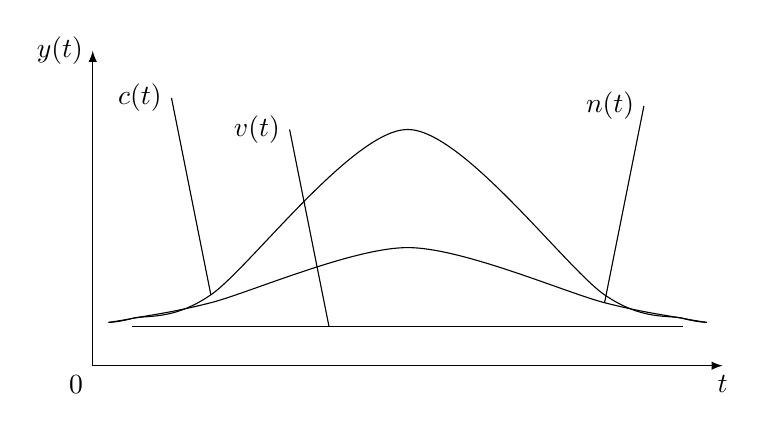
\begin{tikzpicture}

\draw[>=latex,->] (0,0)--(8,0) node[anchor=north] {$t$}; % ось Ox с подписью
\draw[>=latex,->] (0,0)--(0,4) node[anchor=east] {$y(t)$}; % ось Oy с подписью
\draw plot coordinates { (0.5,0.5) (7.5,0.5) };
\draw plot[smooth] coordinates { (0.2,0.55) (0.5,0.6) (1.5,0.9) (4,3) (6.5,0.9) (7.5,0.6) (7.8,0.55) };
\draw plot[smooth] coordinates { (0.2,0.55) (0.5,0.6) (1.5,0.8) (4,1.5) (6.5,0.8) (7.5,0.6) (7.8,0.55) };

\draw plot coordinates { (3,0.5) (2.5,3) } node[anchor=east] {$v(t)$};
\draw plot coordinates { (1.5,0.9) (1,3.4) } node[anchor=east] {$c(t)$};
\draw plot coordinates { (6.5,0.8) (7,3.3) } node[anchor=east] {$n(t)$};
\draw node[anchor=north east] {$0$};


\end{tikzpicture} 
\caption{Наблюдение сигнала с помехой и белым шумом}
\label{fig:man_1}
\end{figure}


Очевидно, что когда уровни полезной составляющей и помеховой составляющей соизмеримы между собой, как это следует из рис. \ref{fig:man_1}, получить удовлетворительное качество оценки затруднительно. 
В этой ситуации уместно использовать адаптивную компенсацию помеховой составляющей $n(t)$.

Необходимо сформировать такой сигнал, который способен уравновесить действие помехового воздействия $n^*(t)\approx-n(t)$ \cite{popovski}, чтобы вычесть его из наблюдаемой реализации:
\begin{equation}\label{eq41:man8}
y^*(t)=c(t)+n(t)-n^*(t)+v(t)=c(t)+v(t)+\Delta n(t),
\end{equation}
\noindent где $\Delta n(t)$ - остаток нескомпенсированной помеховой составляющей (остаточный джиттер).

Однако формированию компенсационного воздействия $n^*(t)$ из основного источника наблюдения (\ref{eq41:man7}) мешает полезная составляющая $c(t)$ и шум наблюдения $\nu (t)$ - уровень которого может быть значительным (рис. \ref{fig:man_1}).
Таким образом, прямого решения нет.
В связи с этим, задача компенсации расширяется и реализовывается в два этапа: вначале находится возможность создания компенсационного сигнала, а потом осуществляется сама компенсация помехи в алгоритме управления наблюдением.


\section{Синтез метода управления буфером компенсации джиттера на основе управления наблюдением системы}

Как упоминалось ранее, из теории автоматического управления известна теорема о разделении \cite{seij, red}, утверждающая о том, что при среднеквадратичном критерии качества и
при гауссовской ситуации, оптимальное управление можно построить из двух раздельных процедур: оптимальной стохастической оценки $\hat x (k)$  и детерминированной процедуры управления:
\begin{equation}\label{eq41:man9}
u(t)=\EuScript{L}(k)\hat x (k),
\end{equation}

Воспользуемся результатами данной теоремы.

Прежде, чем приступить к синтезу методов управления, следует уточнить, каким способом будет осуществляться управление буфером компенсации джиттера поступающих пакетов. 
Очевидно, это может быть реализовано с помощью аддитивной коррекции:
\begin{equation}\label{eq41:man10}
y(k)\pm\hat u(k)
\end{equation}
или мультипликативной коррекции:
\begin{equation}\label{eq41:man11}
y(k)(l\hat u(k)),
\end{equation}
\noindent где $l$ - масштабирующий множитель.

Для разработки методов управления воспользуемся процедурой ФКБ (\ref{eq3:Estim_rel}). Очевидно, для решения задачи необходимо выбрать вариант управления наблюдением (\ref{eq41:man8}),
поскольку именно наблюдаемую величину необходимо корректировать, выбирая или оценивая соответствующую величину коэффициента $H(k)$. 
В литературе \cite{windrow,monzigo} процедуры оценки весовых коэффициентов известны как адаптивные алгоритмы Уидроу-Хоффа. 
Следуя данной литературе, переобозначим $H(k)\equiv W(k)$ и будем находить оптимальную оценку этого коэффициента на основании уравнения (\ref{eq3:Estim_rel}):
\begin{equation}\label{eq41:man12}
\hat W(k+1)=\hat W(k)+A(k)[y(k)-\hat W(k)t_{p}(k)]t_{p}(k),
\end{equation}

Значение $W(k)$ представляет собой комплексный весовой коэффициент, обеспечивающий корректировку фазы компенсации джиттера.

Весовой коэффициент $\hat W(k)$ может быть как вещественным, так и комплексным. 
В первом случае буфер компенсации джиттера обеспечивает процедуру в соответствии с (\ref{eq41:man10}). 
Структурная схема устройства управления, реализующего метод (\ref{eq41:man12}), представлена на рис. \ref{fig:man_2}

\begin{figure}[!h]
\centering
\begin{tikzpicture}        
        [align=center,node distance=2cm]
        \matrix (m1) [row sep=10mm, column sep=15mm] {
		%--------------------------------------------------------------------
		\node[dspnodeopen] (m00) {$y(k)$};    &
		\node[dspadder]                  (m01) {$\sum 1$};          &
		\node[coordinate]                  (m02) {};          &
		\node[coordinate]                  (m03) {};          &
		\node[coordinate]                  (m04) {};          &
		\node[dspnodefull]                  (m05) {$y^*(k)=t_r(k)\pm t_n(k)$};          &
		\node[coordinate]                  (m06) {};          \\
		%--------------------------------------------------------------------
		\node[coordinate]                  (m10) {};          &
		\node[coordinate]                  (m11) {};          &
		\node[coordinate]                  (m12) {};          &
		\node[dspfilter,minimum width=2cm]                  (m13) {$k$};          &
		\node[coordinate]                  (m14) {};          &
		\node[coordinate]                  (m15) {};          &
		\node[coordinate]                  (m16) {};          \\
		%--------------------------------------------------------------------
		\node[coordinate]                  (m20) {};          &
		\node[dspmixer,dsp/label=left]                  (m21) {$m1$};          &
		\node[dspnodefull]                  (m22) {};          &
		\node[coordinate]                  (m23) {};          &
		\node[dspadder,dsp/label=below]                  (m24) {$\sum2$};          &
		\node[dspmixer,dsp/label=right]                  (m25) {$m2$};          &
		\node[coordinate]                  (m26) {};          \\
		%--------------------------------------------------------------------
		\node[coordinate] (m30) {};    &
		\node[dspnodefull]                  (m31) {};          &
		\node[coordinate]                  (m32) {};          &
		\node[coordinate]                  (m33) {};          &
		\node[coordinate]                  (m34) {};          &
		\node[dspfilter,minimum width=2cm,fill=white]                  (m35) {$A(k)$};          &
		\node[coordinate]                  (m36) {};          \\
		%--------------------------------------------------------------------
		\node[coordinate] (m40) {};    &
		\node[dspnodeopen,dsp/label=below]                  (m41) {$t_p(k)$};          &
		\node[coordinate]                  (m42) {};          &
		\node[coordinate]                  (m43) {};          &
		\node[coordinate]                  (m44) {};          &
		\node[coordinate]                  (m45) {};          &
		\node[coordinate]                  (m46) {};          \\
	};
	

\draw[semithick] (m13.0){}+(-0.2,-0.25) -- +(-1.8,-0.25);
\draw[semithick] (m13.0){}+(-0.2,-0.35) -- +(-0.2,-0.15);
\draw[semithick] (m13.0){}+(-1.8,-0.35) -- +(-1.8,-0.15);

\path (m01) node[below left] {$+$} ;
\path (m01) node[below right] {$-$} ;
\path (m13) node[below,yshift=-0.5cm] {ЛЗ} ;
\path (m24) node[above right] {$\hat W(k)$} ;
\path (m21) node[below right] {$\hat W(k+1)$} ;
\path (m11) node[yshift=0.5cm] {$u(k)=t_p\times \hat W(k+1)$} ;

	\begin{scope}[start chain]
		\chainin (m00);
		\chainin (m01) [join=by dspconn];
		\chainin (m06) [join=by dspconn];

	\end{scope}
	
	\begin{scope}[start chain]
		\chainin (m05);
		\chainin (m25) [join=by dspconn];
		\chainin (m24) [join=by dspconn];
		\chainin (m21) [join=by dspconn];
		\chainin (m01) [join=by dspconn];
	\end{scope}
	
	\begin{scope}[start chain]
		\chainin (m22);
		\chainin (m12) [join=by dspline];
		\chainin (m13) [join=by dspconn];
		\chainin (m14) [join=by dspline];
		\chainin (m24) [join=by dspconn];

	\end{scope}
	\draw[dspconn] (m41) -- (m21);
	\draw[dspconn] (m31) -- (m35);
	\draw[dspconn] (m35) -- (m25);
	
        \end{tikzpicture}
\caption{Метод управления буфером компенсации джиттера с аддитивной коррекцией}
\label{fig:man_2}
\end{figure}

Аналогично предыдущему методу также можно построить управление буфером компенсации джиттера с мультипликативной коррекцией (рис. \ref{fig:man_3})

\begin{figure}[!h]
\centering
\begin{tikzpicture}        
        [align=center,node distance=2cm]
        \matrix (m1) [row sep=10mm, column sep=20mm] {
		%--------------------------------------------------------------------
		\node[dspnodeopen] (m00) {$y(k)$};    &
		\node[dspnodefull,dsp/label=left]                  (m01) {};          &
		\node[dspmixer]                  (m02) {$m1$};          &
		\node[coordinate]                  (m03) {};          &
		\node[dspnodefull]                  (m04) {$y^*(k)=t_r(k)\pm t_n(k)$};          &
		\node[coordinate]                  (m05) {};          \\
		%--------------------------------------------------------------------
		\node[coordinate]                  (m10) {};          &
		\node[coordinate]                  (m11) {};          &
		\node[dspnodefull]                  (m12) {};          &
		\node[coordinate]                  (m13) {};          &
		\node[coordinate]                  (m14) {};          &
		\node[coordinate]                  (m15) {};          \\
		%--------------------------------------------------------------------
		\node[coordinate]                  (m20) {};          &
		\node[coordinate]                  (m21) {};          &
		\node[coordinate]                  (m22) {};          &
		\node[dspfilter,minimum width=2cm]                  (m23) {$k$};          &
		\node[dspadder,dsp/label=left]                  (m24) {$\sum 2$};          &
		\node[dspnodeopen]                  (m25) {$t_p(k)$};          \\
		%--------------------------------------------------------------------
		\node[coordinate] (m30) {};    &
		\node[coordinate]                  (m31) {};          &
		\node[dspadder,dsp/label=left]                  (m32) {$\sum 1$};          &
		\node[coordinate]                  (m33) {};          &
		\node[coordinate]                  (m34) {};          \\
		%--------------------------------------------------------------------
		\node[coordinate] (m40) {};    &
		\node[dspfilter,minimum width=2cm]                  (m41) {$A(k)$};          &
		\node[dspmixer,dsp/label=below]                  (m42) {$m2$};          &
		\node[coordinate]                  (m43) {};          &
		\node[coordinate]                  (m44) {};          \\
	};
	
	\draw[semithick] (m23.0){}+(-0.2,-0.25) -- +(-1.8,-0.25);
	\draw[semithick] (m23.0){}+(-0.2,-0.35) -- +(-0.2,-0.15);
	\draw[semithick] (m23.0){}+(-1.8,-0.35) -- +(-1.8,-0.15);
	
	\path (m23) node[below right,yshift=-0.5cm] {ЛЗ} ;
	\path (m32) node[below right] {$\hat W(k)$} ;
	\path (m12) node[below right] {$\hat W(k+1)$} ;
	\path (m12) node[above right] {$u(k)\equiv \hat W(k)$} ;
	
		\begin{scope}[start chain]
		\chainin (m00);
		\chainin (m02) [join=by dspconn];
		\chainin (m05) [join=by dspconn];

		\end{scope}
		\begin{scope}[start chain]
		\chainin (m01);
		\chainin (m41) [join=by dspconn];
		\chainin (m42) [join=by dspconn];
		\chainin (m32) [join=by dspconn];
		\chainin (m12) [join=by dspline];
		\chainin (m13) [join=by dspline];
		\chainin (m23) [join=by dspconn];
		\chainin (m33) [join=by dspline];
		\chainin (m32) [join=by dspconn];
		\end{scope}
		\begin{scope}[start chain]
		\chainin (m04);
		\chainin (m24) [join=by dspconn];
		\chainin (m44) [join=by dspline];
		\chainin (m42) [join=by dspconn];

		\end{scope}
		
		\draw[dspconn] (m25) -- (m24);
		\draw[dspconn] (m12) -- (m02);
		
        \end{tikzpicture}
\caption{Метод управления буфером компенсации джиттера с мультипликативной коррекцией}
\label{fig:man_3}
\end{figure}

Метод работает следующим образом. 
Время задержки каждого прибывшего пакета поступает на сумматор $\sum 1$. 
На второй вход этого устройства поступает управляющий сигнал $u(k)$, который содержит информацию о том, на сколько следует скорректировать задержку прибытия пакета:

\begin{equation}\label{eq41:man13}
u(k)=t_p(k)\times \hat W(k+1),
\end{equation}

\noindent где $t_p(k)$ - ожидаемое время воспроизведения, которое состоит из двух составляющих: интервала между пакетами, полученного из заголовков пакета с помощью спецификации кодека передачи и начального смещения $\Delta t^i$ (рис. \ref{fig:man_4}), которое и является, на практике, размером буфера компенсации джиттера.
Поскольку задержка $y(k)$ носит случайный характер, то на выходе $\sum 1$ всегда будет иметь место остаточная расстройка фазы $\pm t_n(k)$.
Сигнал этой расстройки поступает на перемножитель $m2$ на второй вход его поступает сигнал о фазе опорного сигнала $t_p(k)$. 
В результате перемножения на выходе $m2$ имеем:
\begin{equation}\label{eq41:man14}
U_{m2}=(U_{tr}+U_{tn})U_{tp}=U_{tr}U_{tp}+U_{tn}U_{tp}.
\end{equation}

После интегрирования все слагаемые, кроме последнего, в среднем равны нулю, поскольку они не коррелированы между собой.
\begin{equation}\label{eq41:man15}
U_u=\int U_{tn}U_{tp}dt\neq0.
\end{equation}
Полученное управление (\ref{eq41:man15}) является, по сути, сигналом весового коэффициента:
\begin{equation}\label{eq41:man16}
u(k)\equiv \hat W(k+1).
\end{equation}

В результате действия такой кольцевой схемы с обратной связью постепенно уменьшается остаточная задержка $t_n(k)$ и после некоего минимального значения наступает стабилизация.

Данная структура (рис. \ref{fig:man_2}) используется многими специалистами и хорошо зарекомендовала себя на практике в алгоритмах управления адаптивными решетками (ААР) \cite{popovski,monzigo,windrow}.

Близкой по принципу является работа другой адаптивной схемы (рис. \ref{fig:man_3}).
Здесь сигнал рассогласования $U_{tn}$ между $t_p(k)$ и $t_r$ формируется на выходе сумматора $\sum 2$. 
Далее на выходе перемножителя $m2$ образовывается суммарный сигнал рассогласования фаз, аналогичный рис. \ref{fig:man_2} и после интегратора ($\sum1$ и ЛЗ) формируется весовой коэффициент $\hat W(k+1)$, мультипликативно воздействующий на устройство $m1$, содержащий корректор фазы последовательности $t_r(k)$ до тех пор, пока на выходе $\sum2$ будет действовать сигнал рассогласования фаз $t_n(k)$.



\begin{figure}[!h]
\centering
\begin{tikztimingtable}[
    timing/slope=0,         % no slope
    timing/coldist=2pt,     % column distance
    xscale=2.05,yscale=1.1, % scale diagrams
    thick               % set line width
  ]
  $t_s(k)$ &R 0.2L 6{2QL} \\
  \\
  \\
  \\
  $y(k)$&R  2.2L 2Q 0.8L 2Q 1.2L 2Q 0.2L 2Q 3.8L 2Q 0.1L \\
    \\
  \\
  $t_p(k)$ &[densely dashed]R 3.2L 5{2QL} \\
  $y(k)\pm u(k)$&R  3.2L 4{2QL} L 2U 0.1L\\
  \extracode
  
  \begin{pgfonlayer}{background}
\draw[densely dashed] (0.2,0) --+(2,-8);
\draw[densely dashed] (2.2,0) --+(2.8,-8);
\draw[densely dashed] (5.2,0) --+(3,-8);
\draw[densely dashed] (8.2,0) --+(2.2,-8);
\draw[densely dashed] (11.2,0) --+(5,-8);

\draw[densely dashed] (2.2,-8) --+(0,-8);
\draw[densely dashed] (5,-8) --+(0,-8);
\draw[densely dashed] (8.2,-8) --+(0,-8);
\draw[densely dashed] (10.4,-8) --+(0,-8);
\draw[densely dashed] (16.25,-8) --+(0,-8);

\draw (2.2,-16) --+(0,-1);
\draw (3.19,-16) --+(0,-1);
\draw (2.0,-16.7) --+(1.4,0);
\draw[>=latex,->] (1.8,-16.7) --+(0.4,0);
\draw[>=latex,->] (3.6,-16.7) --+(-0.4,0);
\path (2.7,-16.7) node[below] {$\Delta t^i$} ;

  \end{pgfonlayer}
\end{tikztimingtable}
\caption{Управление буфером компенсации джиттера с помощью предложенных методов}
\label{fig:man_4}
\end{figure}


Размер буфера $\Delta t^i$ рассчитывается только для первого пакета каждого речевого потока на основе оценки отклонения $\hat V (k)$ от условного среднего значения сетевой задержки (\ref{eq3:syntes1}-\ref{eq3:syntes2}):
\begin{equation}\label{eq41:syntes3}
\hat{V}(k)=\alpha\cdot\hat{V}(k-1)+(1-\alpha)\cdot V(k),
\end{equation}

\begin{equation}\label{eq41:syntes4}
V^i(k)= \;
\begin{cases}
| \hat{x}(k)-x(k) |, \; K(k)\Delta y \leq b; \\    
V(k-1), \;  K(k)\Delta y > b,    
\end{cases}
\end{equation}

\begin{equation}\label{eq41:syntes5}
\Delta t^i= \;
\begin{cases}
\gamma\cdot\hat{V}^{i-1}, \; \hat{V}^{i-1} \geq \Delta t_{min}; \\    
\gamma\cdot\Delta t_{min}, \;  \hat{V}^{i-1} < \Delta t_{min},    
\end{cases}
\end{equation}
\noindent где $\gamma$ - константа для управления процентом отбрасываемых пакетов и задержкой.


\section{Синтез метода управления буфером компенсации джиттера на основе оценки джиттера ГРФКБ}

Полученный метод управления, изображенные на рис. \ref{fig:man_3}-\ref{fig:man_2} обладает рядом недостатков:
\begin{itemize}
 \item Рассчитан на работу с входящим воздействием гауссовского распределения, в то время, как у нас сугубо не линейная задача.
 \item Полученный метод управления является чрезмерно усложненным по сравнению с простыми методами управления буфером, которые уже реализованы на практике \cite{Moon,jesuspinto1999algorithms,YoungJongChoChongKwanUn19941385,DBLP:journals/iet-com/Gade07,Hafskjold:2003:AAO:963600.963677}.  
\end{itemize}

Вследствие чего рассмотрим более простой метод управления буфером (рис. \ref{fig:man_5}).

\begin{figure}[!h]
\centering
\begin{tikzpicture} 
[align=center,node distance=2cm]
        \matrix (m1) [row sep=10mm, column sep=20mm] {
		%--------------------------------------------------------------------
		\node[dspnodeopen] (m00) {};    &
		\node[dspfilter,minimum size=2cm,text height=2em]                  (m01) {Предварительный \\обработчик};          &
		\node[dspfilter,minimum width=2cm]                  (m02) {Буфер};          &
		\node[coordinate]                  (m03) {};          \\
		%--------------------------------------------------------------------
		\node[coordinate]                  (m10) {};          &
		\node[dspfilter,minimum width=2cm]                  (m11) {ГРФКБ};          &
		\node[dspfilter,minimum width=2cm]                  (m12) {Контроллер};          &
		\node[dspfilter,minimum width=2cm]                  (m13) {Плейер};          \\
		%--------------------------------------------------------------------
		\node[coordinate]                  (m20) {};          &
		\node[coordinate]                  (m21) {};          &
		\node[dspnodeopen,dsp/label=below]                  (m22) {$b, \gamma, \Delta t_{min}$};          &
		\node[coordinate]                  (m23) {};          \\
	};
		\begin{scope}[start chain]
		\chainin (m00);
		\chainin (m01) [join=by dspconn];
		\chainin (m02) [join=by dspconn];
		\chainin (m12) [join=by dspconn];
		\chainin (m13) [join=by dspconn];
		\end{scope}
		\begin{scope}[start chain]
		\chainin (m01);
		\chainin (m11) [join=by dspconn];
		\chainin (m12) [join=by dspconn];
		\end{scope}
		\draw[dspconn] (m22) -- (m12);
		\timing [yshift=0.3cm] (m00) {0.2lz0.3lz2lz2lz0.1lz};
		\timing [yshift=0.3cm,xshift=2.3cm] (m01) {0.2lz0.3lz2lz2lz0.1lz};
		\timing [yshift=0.3cm,xshift=1.7cm] (m12) {3{lz}l};
		\path (m01) node[below right,yshift=-1cm] {$t_r(k)$} ;
		\path (m11) node[above right,xshift=1.5cm] {$\hat x(k+1)$} ;
\end{tikzpicture}
\caption{Блок схема метода управления буфером компенсации джиттера}
\label{fig:man_5}
\end{figure}

На рис. \ref{fig:man_5} пакеты прибывают на блок предварительной обработки, где анализируются заголовки пакетов, после чего принимается решение о помещение пакета в буфер.
Полученные временные характеристики пакета передаются на блок ГРФКБ, где производится оценка текущего джиттера задержки для конкретного потока данных.
Основное управление производится на контроллере: 
\begin{itemize}
 \item Определяются речевые потоки.
 \item На основе оценки полученной от ГРФКБ (\ref{eq3:syntes1}-\ref{eq3:syntes2}) и данных определенных администратором системы рассчитывается размер буфера для первого пакета в речевом потоке.
 \item Если предварительная статистика отсутствует или устарела, то для первого пакета в речевом потоке устанавливается размер буфера по умолчанию.
 \item Для всех остальных пакетов размер буфера детерминировано рассчитывается на основе времени воспроизведения первого пакета этого речевого потока и интервала между пакетами, который был определен во время передачи.
\end{itemize}


\section{Выводы по четвертому разделу}
\begin{enumerate}

 \item
 %Для синтеза алгоритма управления джиттером предложено использовать условия определенные теоремой о разделении,
 %при которой процедура оптимального управления определяется в виде двух отдельных процедур:
 %стохастической оценки и детерминированного управления.
 %Предложено использовать алгоритмы управления двух видов:
 %управление состоянием и управление наблюдением.
 В соответствии с теорией об оптимальном управлении, управление может быть реализовано с помощью двух методов:
 управление наблюдением и управление состоянием.
 В работе рассмотрены оба эти метода.
 В алгоритме управления состоянием полученная оценка текущего состояния джиттера воздействует непосредственно на указанное состояние и соответствующим образом корректирует его.
 В алгоритме управления наблюдением предполагается осуществление автоматического 
 слежения за состоянием процесса джиттера с тем, чтобы временной зазор между генерируемой 
 последовательностью пакетов на стороне отправителя и получаемой последовательностью на стороне получателя оставался минимальный.
 
 %При выборе традиционного для ТКС среднеквадратичного критерия уместно воспользоваться теоремой о разделении и структуру этого метода выбрать в виде двух различных блоков:
 %оптимальное стохастическое оценивание и детерминированное управление.
  \item Для синтеза алгоритма управления буфером компенсации джиттера целесообразно выбрать метод автоматического управления, функционирующего по принципу Уатта. 
 Сама компенсация при этом относится к классу управления наблюдением.
 \item Функционирование метода компенсации джиттера основано на компенсационной процедуре при которой фаза первого пакета $n$-ого речевого потока выбирается на основании статистики наблюдаемой в канале.
 \item В качестве управляемого объекта в методе компенсации джиттера используется комплекс весовых коэффициентов, подстраивающих фазу приходящей из линии последовательности пакетов к фазе опорной последовательности.
 \item Предложено два метода управления алгоритмом компенсацией джиттера за счет преобразования базиса наблюдения, обеспечивающих возможность использования для аддитивной и мультипликативной коррекции фазы джиттера.
 \item Предложена более простой адаптивный метод управления алгоритмом компенсацией джиттера, позволяющий формировать буфер для каждого речевого потока, который и будет использован в дальнейшем для моделирования и анализа эффективности для предложенного метода.
\end{enumerate}
